\documentclass[a4paper,11pt]{article}
\usepackage{xcolor}
\usepackage{caption}
\usepackage{tikz}
\usepackage{tkz-euclide}
\usetikzlibrary{intersections,shapes.arrows,arrows.meta}
\begin{document}
\begin{figure}[H]
\begin{center}
\def\radius{6mm}
\scalebox{0.4}{
 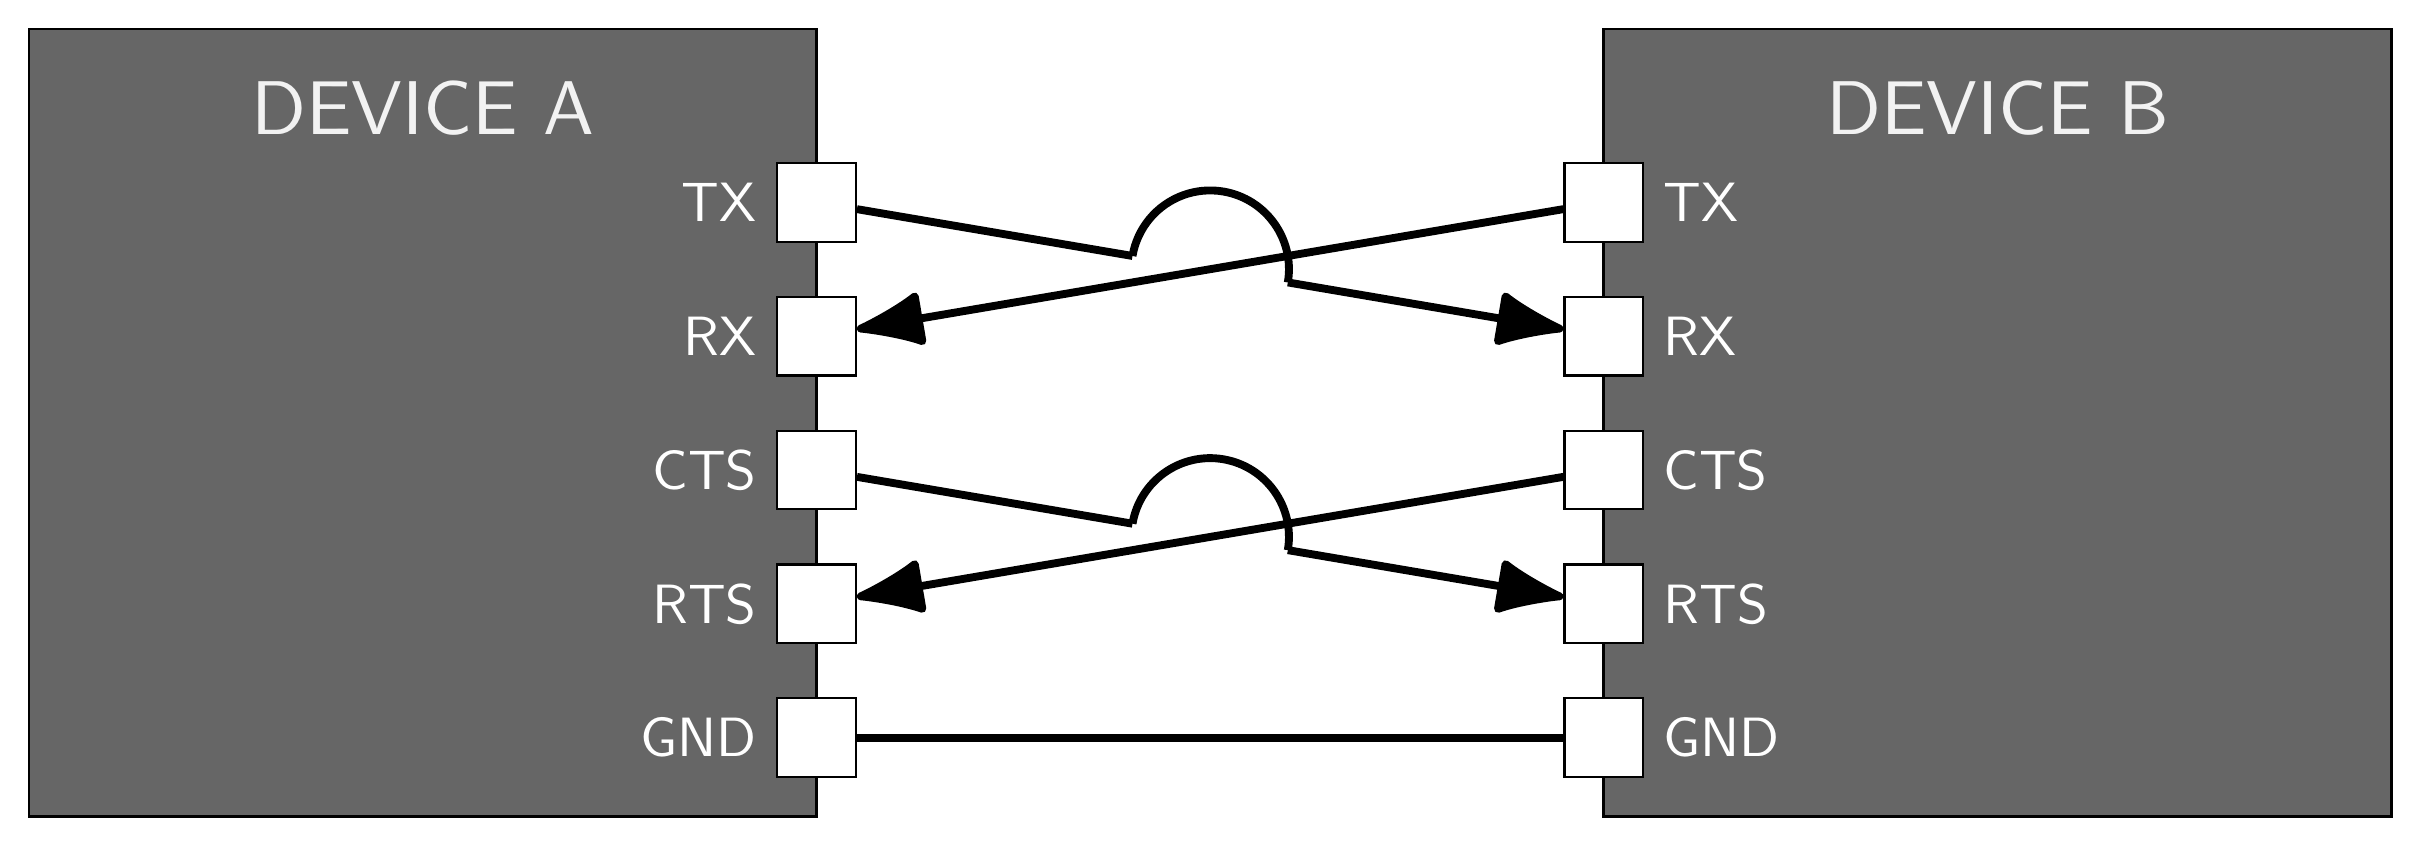
\begin{tikzpicture}[font=\sffamily]
	\draw[line width=1, fill=black!60] (0,0) rectangle ++(10,10);
	\draw[line width=1, fill=black!60] (20,0) rectangle ++(10,10);
	\draw (5,9) node[scale=2.75,black!5]{DEVICE A};
	\draw (25,9) node[scale=2.75,black!5]{DEVICE B};

	\foreach \p [count=\q from 0] in {{GND},{RTS},{CTS},{RX},{TX}}{
		\node (rect) at (10, 1+\q*1.7) [draw,thick,minimum width=1cm,minimum height=1cm,fill=white,label={[white,scale=2] left:\p}] (l-\p){};
		\node (rect) at (20, 1+\q*1.7) [draw,thick,minimum width=1cm,minimum height=1cm,fill=white,label={[white,scale=2] right:\p}] (r-\p){};
	}

	\draw [-{Latex[length=1cm, round]},line width=1mm,name path=line 1] (r-TX) -- (l-RX);
	\path[name path=line 2] (l-TX) -- (r-RX);
	\path [name intersections={of = line 1 and line 2, name=i}];
	\coordinate (S) at (i-1);
	\path[name path=c1] (S) circle(\radius);
	\path [name intersections={of = c1 and line 2, name=i}];
	\coordinate (I1)  at (i-2);
	\coordinate (I2)  at (i-1);
	\draw[line width=1mm] (l-TX) -- (I2);
	\draw[-{Latex[length=1cm, round]},line width=1mm] (I1) -- (r-RX);
	\tkzDrawArc[line width=1mm](S,I1)(I2);

	\draw [-{Latex[length=1cm, round]},line width=1mm,name path=line 3] (r-CTS) -- (l-RTS);
	\path[name path=line 4] (l-CTS) -- (r-RTS);
	\path [name intersections={of = line 3 and line 4, name=i}];
	\coordinate (T) at (i-1);
	\path[name path=c2] (T) circle(\radius);
	\path [name intersections={of = c2 and line 4, name=i}];
	\coordinate (I3)  at (i-1);
	\coordinate (I4)  at (i-2);
	\draw[line width=1mm] (l-CTS) -- (I3);
	\draw[-{Latex[length=1cm, round]},line width=1mm] (I4) -- (r-RTS);
	\tkzDrawArc[line width=1mm](T,I4)(I3);

	\draw [line width=1mm] (l-GND) -- (r-GND);

	\end{tikzpicture}
 }
 \captionof{figure}{Hardware flow control.}
 \label{fig:flowctl}
\end{center}
\end{figure}
\end{document}



